\documentclass{scrartcl}

\usepackage[ngerman]{babel}

\usepackage[utf8]{inputenc}
\usepackage{hyperref,xcolor,microtype,ifthen}
\usepackage{csquotes}

\usepackage{graphicx}
\usepackage{svg}

\usepackage{helvet}
\renewcommand{\familydefault}{\sfdefault}
\fontfamily{phv}\selectfont

\linespread{1.25}

\begin{document}

\section{Einleitung}
\subsection{Motivation}
\subsection{Ziel}
\subsection{Aufbau}

\section{Grundlagen}
\subsection{Quartettspiel}
\subsection{Mobile Plattform}
\subsection{Frameworks}

\section{Anforderungsanalyse}
\subsection{Funktionale Anforderungen}

Im folgenden werden alle funktionalen und nicht funktionalen Anforderungen
aufgelistet, die vor oder während der Entwicklung der Applikation gestellt wurden.

\ \newline
\textbf{FA1 Hauptmenü} \newline
Der Benutzer kann von einem Hauptmenü, welches nach Start der App angzeigt wird,
schnell auf die wichtigsten Funktionen der App zugreifen.

\ \newline
\textbf{FA2 Spielmodi} \newline
Der Benutzer kann vor jedem Spiel aus 4 verschiedenen Spielmodi wählen: Zeitspiel
(Spielende nach Ablauf eines Zeitlimits), Punktspiel (Spielende bei bestimmter
Punktezahl), Rundenspiel (Spielende nach bestimmer Anzahl Runden), Insane
(Vergleiche umgekehrt, Spielende nach bestimmter Anzahl Runden).

\ \newline
\textbf{FA3 Computergegner} \newline
Im Einzelspieler Modus kann der Benutzer gegen einen simulierten Gegner antreten.
Dieser sollte sich wie ein menschlicher Spieler verhalten und nicht auf
Informationen zurückgreifen können die einem menschlichen Gegner normalerweise
nicht zur Verfügung stehen. So sollte z.B. die Werte der Karte des Benutzers dem
Computergegner nicht für die Planung des Spielzugs zur Verfügung stehen. So soll
ein \enquote{unfaires} Verhalten und damit ein frustrierendes Spielerlebnis
verhindert werden.

\ \newline
\textbf{FA4 Schwierigkeitsgrad} \newline
Vor jedem neuen Spiel kann der Benutzer einen von 3 verschiedene
Schwierigkeitsgraden (Leicht, Mittel, Schwer) wählen. Je nach gewähltem
Schwierigkeitsgrad handelt der Computergegner mehr oder weniger intelligent.

\ \newline
\textbf{FA5 Spiel fortsetzen} \newline
Der gesamte Spielfortschritt wird kontinuierlich in der Applikation persistent
gespeichert. So kann auch nach einem Neustart der App das Spiel ohne
Fortschrittsverlust fortgesetzt werden.

\ \newline
\textbf{FA6 Gallerie} \newline
Alle im Spiel vorhandenen Quartettdecks lassen sich in einer speziellen Ansicht,
der Gallerie, betrachten. Dabei können alle im Deck enthaltenen Karten einzeln
in einer detaillierten Ansicht betrachtet werden.

\ \newline
\textbf{FA7 Deck Download} \newline
Die Applikation erlaubt das Herunterladen weiterer Kartendecks von einem
externen Server. Nach dem Herunterladen können diese Decks genauso wie die
bereits in der App vorhandenen Decks im Spiel verwendet werden. Die Decks werden
persistet gespeichert und sind somit nach erfolgreichem Download auch ohne
Internetverbindung dauerhaft verfügbar.

\ \newline
\textbf{FA8 Statistiken} \newline
Die App sammelt während der Laufzeit spielbezogene Daten, um Statistiken zu
ermöglichen. Diese Statistiken können vom Spieler in einer speziellen Ansicht
eingesehen werden. Mögliche Statistiken sind: kill / death ratio, höchste
Gewinnserie, höchste Verlustserie

\ \newline
\textbf{FA9 Rangliste} \newline
Es gibt eine Rangliste, in welcher der Benutzer die im Spiel erhaltenen Punkte
mit seinem Namen publizieren kann.

\ \newline
\textbf{FA10 Achievements} \newline
Die App beinhaltete ein Achievementsystem. Wenn gewissen Herausforderungen
erfüllt werden können Achievements freigeschaltet werden und in einer speziellen
Ansicht angesehen werden.

\ \newline
\textbf{FA11 Quartetteditor} \newline
Es wird ein Quartetteditor bereitgestellt, der es dem Benutzer ermöglich
eigene Quartettdecks zu erstellen. Mit den erstellen Decks kann wie mit den
bereits im Spiel integrierten Decks gespielt werden.

\ \newline
\textbf{FA12 Levelsystem} \newline
Ein Levelsystem suggeriert permanenten Fortschritt. Nach jedem Spiel erhält der
Benutzer Erfahrungspunkte, welche das Level steigen lassen. Mit diesem System
soll eine Langzeitmotivation erreicht werden.

\ \newline
\textbf{FA13 Multiplayer} \newline
Es ist über ein Netzwerk möglich gegen andere Benutzer der App anzutreten.


\subsection{Nichtfunktionale Anforderungen}

\textbf{NFA1 Robustheit} \newline
Das Spiel soll eine gewisse Robustheit aufweisen, also auf fehlerhafte Eingaben
oder unvorhergesehene Ereignisse angemessen reagieren. Im Falle eine Absturzes
sollte die Applikation ohne Verlust des Spielfortschritts neu gestartet werden
können.

\ \newline
\textbf{NFA2 Erweiterbarkeit} \newline
Die Programmstruktur der Applikation sollte derart gestaltet sein, dass
spätere Erweiterungen möglichst einfach vorgenommen werden können.

\ \newline
\textbf{NFA3 Responsiveness} \newline
Die Oberfläche sollte stehts innerhalb einer sehr kurzen Zeit auf
Benutzereingaben reagieren. Bei längeren Wartezeiten, etwa während eines
Downloads, sollte der Benutzer permanent, durch den Einsatz von entsprechenden
GUI-Elementen, über den Fortschritt der Operation informiert werden.

\ \newline
\textbf{NFA4 Usability} \newline
Der Benutzer sollte die App, nach einer kurzen Einführung, duch eine intuitive
und benutzerfreundliche Oberfläche ohne weitere Anleitung bedienen können.

\section{Konzept und Entwurf}
\subsection{Mockups}

\newpage
\section{Implementierung}
\subsection{Ausgewählte Implementierungsdetails}
\subsubsection{Gallerie}

\begin{figure}
  \centering
  \begin{minipage}{0.45\textwidth}
    \centering
    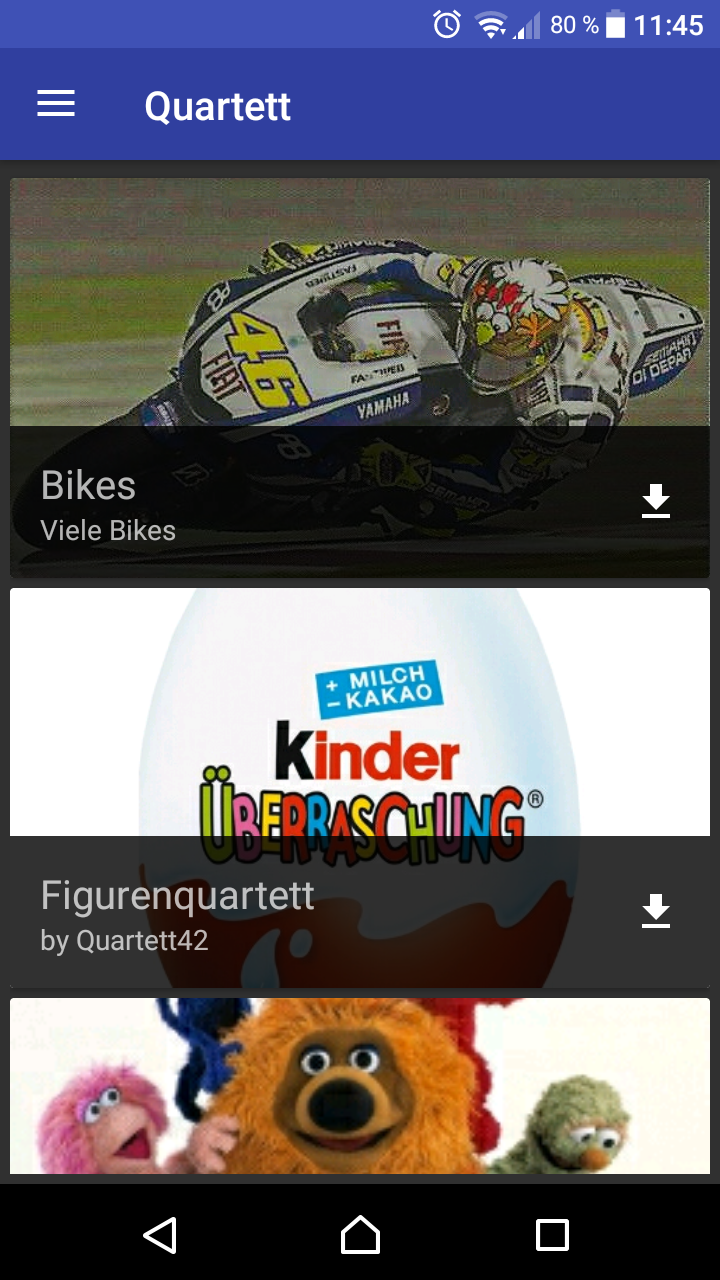
\includegraphics[width=4cm]{img/gallery_decks.png}
    \caption{Deckansicht}
  \end{minipage}
  \hfill
  \begin{minipage}{0.45\textwidth}
    \centering
    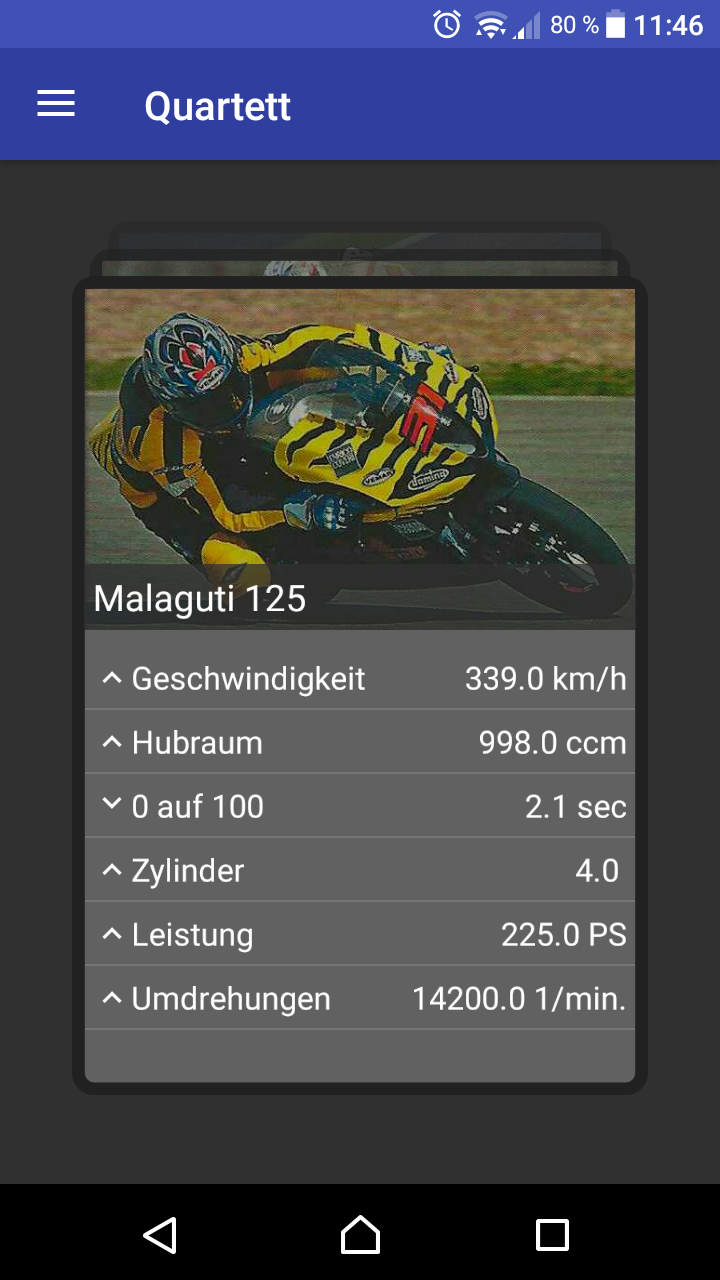
\includegraphics[width=4cm]{img/gallery_cards.png}
    \caption{Kartenansicht}
  \end{minipage}
\end{figure}

\noindent
In der Gallerie werden alle Kartendecks aufgelistet, die auf dem Smartphone
vorhanden sind oder vom Server heruntergeladen werden können. Heruntergeladenen
Decks könne durch Antippen geöffnet werden. In der geöffneten Ansicht kann der
Benutzer durch vertikale Wischgesten durch die einzelnen Karten des virtuellen
Kartenstapels blättern. Tippt der Benutzer ein Deck an, welches nicht
heruntergeladen ist, wird ein Dialog geöffnet in welchem das Herunterladen des
Decks bestätigt oder abgelehnt werden kann. Das Deck wird nicht direkt geladen,
da sich der Benutzer eventuell in einer Netzwerkumgebung befindet in welcher
durch Downloads Kosten entstehen können. Durch den Bestätigungsdialog wird dem
Benutzer somit eine Möglichkeit gegeben den Download zu einem späteren Zeitpunkt
mit günstigeren Netzwerkbedingungen zu starten. Wird der Dialog bestätigt startet
der Download des Decks. Im Listenelement des Decks wird ein Ladebalken angezeigt
und im Notification Drawer wird eine Notification erstellt die ebenfalls den
Fortschritt des Downloads anzeigt. Nach erfolgreichem Download wird die
Notification geschlossen und der Ladebalken verschwindet wieder. Das Deck ist
dann persistent auf dem Gerät gespeichert und kann nun auch ohne
Internetverbinung angezeigt werden. Zudem können nun auch die Karten des Decks,
wie oben beschreiben angezeigt werden. Auch kann das Deck nun im Einzelspieler
Modus verwendet werden.

\begin{figure}
  \centering
  \begin{minipage}{0.45\textwidth}
    \centering
    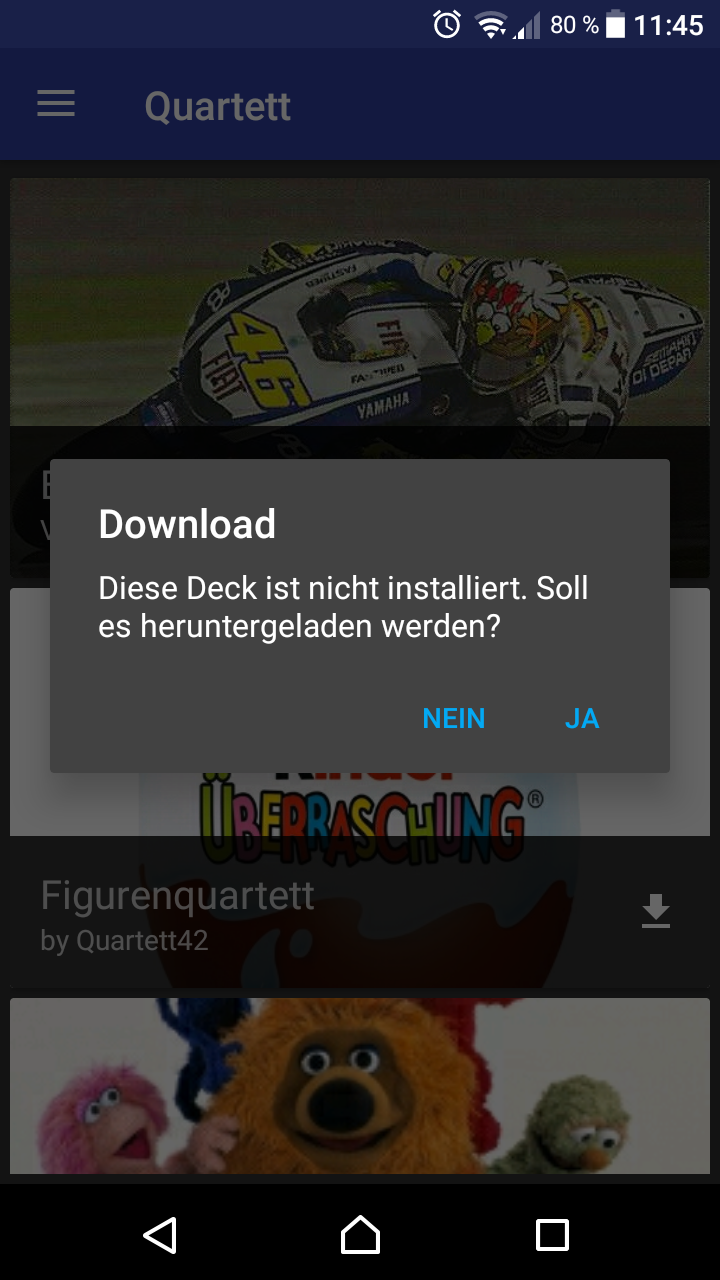
\includegraphics[width=4cm]{img/gallery_dialog.png}
    \caption{Deckansicht}
  \end{minipage}
  \hfill
  \begin{minipage}{0.45\textwidth}
    \centering
    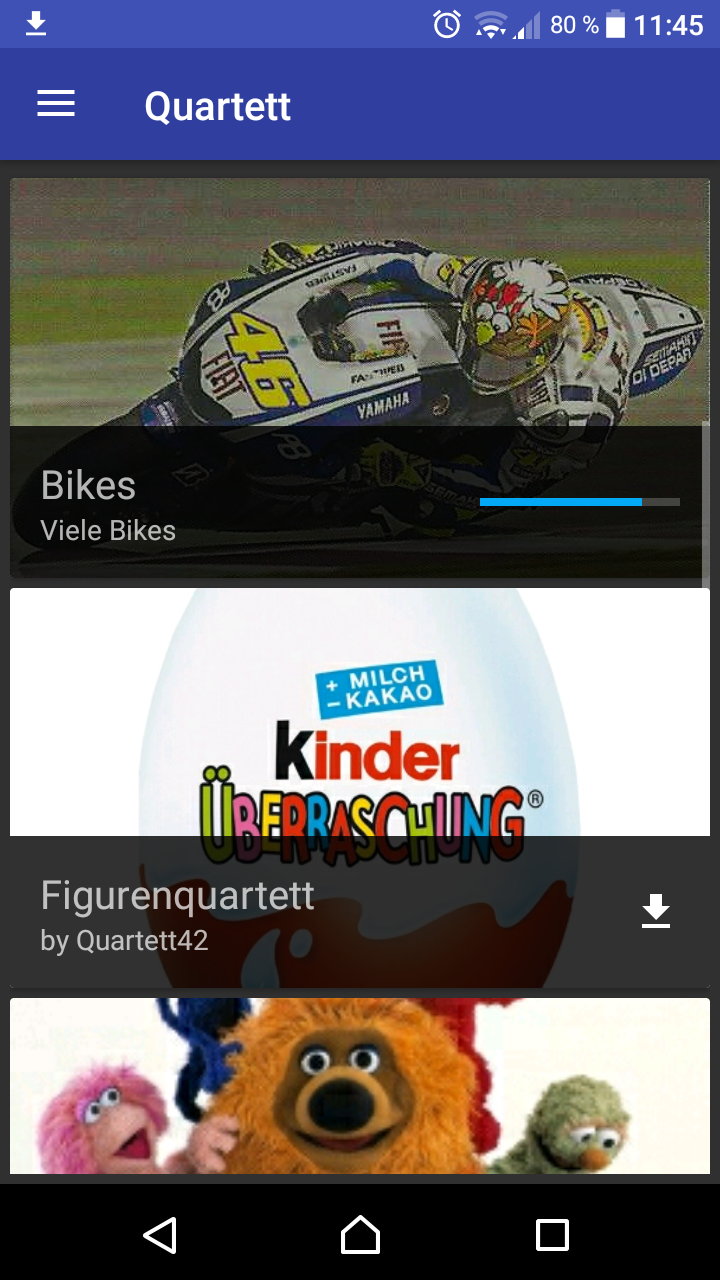
\includegraphics[width=4cm]{img/gallery_download.png}
    \caption{Kartenansicht}
  \end{minipage}
\end{figure}

\ \newline
Um die Gallerie mit diesen beschriebenen Funktionen zu
realisieren waren einige besondere Implementierungsmethoden notwendig. Da den
meisten Decks und Karten relativ hoch auflösendede Bilder zugeordnet sind,
entstehen beim Anzeigen der Decks bzw. Karten Verzögerungen, da große
Datenmengen geladen werden müssen. Dabei ist außerdem zu erwähnen, dass das
Laden der Bilder der Decks, die nicht auf dem Gerät gespeichert sind, über das
Netzwerk erfolgt und somit zusätzliche Verzögerungen entstehen. All diese
Verzögerungen sind als starke Ruckler bemerkbar und beinträchtigen das
Nutzererlebnis erheblich. Das Laden der Bilder wurde daher auf einen zweiten
Thread ausgelagert. Somit kann der Benutzer weitere Interaktion vornehmen
während im Hintergrund die Bilder nachgeladen werden. Auch der Download eines
Decks verwendet einen eigenen Thread, um Verzögerungen im Hauptthread der
Applikation zu vermeiden. Zusätzlich wurde hier auch das Service Modell der
Android Platform verwendet. So kann garantiert werden, dass der Download
abgeschlossen wird, auch wenn die Gallerie verlassen oder die App während des
Downloads geschlossen wird. Um die heruntergeladenen Daten in der Datenbank zu
speichern war ebenfalls eine besonderer Strategie nötig. Die Daten können nicht
sofort gespeichert werden, da sonst bei Fehlern inkonsistente Zustände in der
Datenbank auftreten. Daher werden geladene Daten zunächst im RAM gehalten
bis der Download vollständig abgeschlossen ist und dann in einer einzigen
Transaktion in die Datenbank geschrieben. Somit wird immer ein konsistenter
Zustand der Datenbank erreicht und Fehler können einfacher abgefangen werden.

\subsubsection{Einzelspieler}
\subsubsection{Multiplayer}
\subsection{Architektur}
\subsubsection{Datenmodell}

\begin{figure}[h]
  \centering
  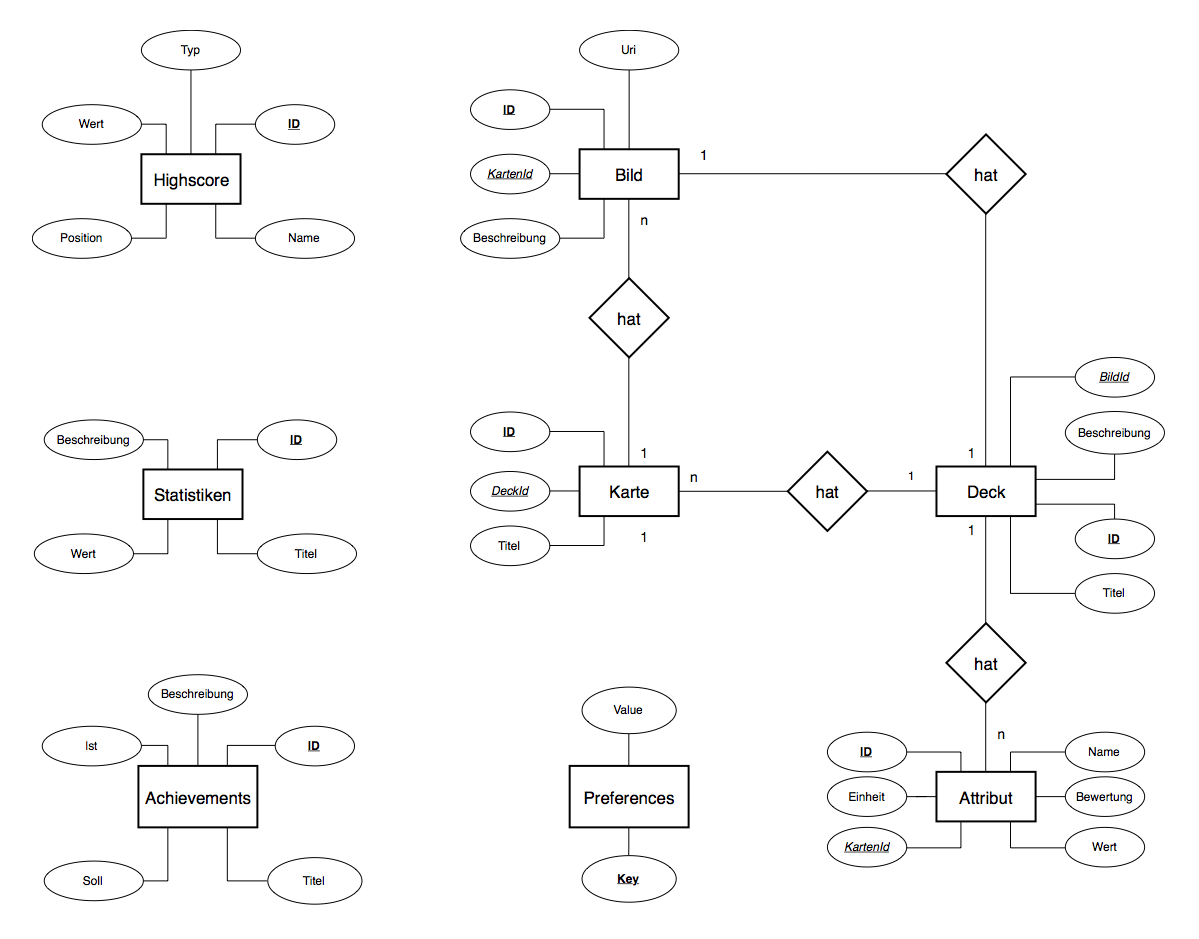
\includegraphics[width=\textwidth]{img/map_er.png}
  \caption{ER Diagramm des Datenmodells}
\end{figure}

\noindent
Im obigen ER Diagramm ist die Struktur unseres Datenmodells dargestellt. Zur
Realisierung wurde die in Android integrierte SQL Datenbank SQLite in
Kombination mit Sugar ORM verwendet. So konnte die einzelnen Entitäten direkt
über Klassen angesprochen werden und es mussten keine SQL Statements verwendet
werden. Allerdings beherrscht Sugar ORM in der verwendeten Version keine Listen
und Beziehungen zwischen den einzelnen Eintitäten können mit Sugar ORM ebenfalls
nur schwierig oder gar nicht dargestellt werden. Die Daten der gespeicherten
Bilder wurden nicht in die SQL Datenbank geladen sondern direkt im internen
Speicher des Geräts abgelegt. Auch die \enquote{Preferences} werden nicht mit
SQL gespeichert sondern in den SharedPreferences des Android Systems abgelegt.
SharedPreferences ist eine einfach Key-Value Datenbank für kleine Datenmengen,
wie z.B. die Einstellungen einer App.

\subsubsection{Klassenstruktur}
\subsection{Besonderheiten}
\subsubsection{Model-View-Presenter}
\section{Anforderungsabgleich}


\end{document}
